% document class and packages
\documentclass{beamer}
\usepackage{algorithm,algorithmic}
\usepackage{amsmath}
\usepackage{amssymb}
\usepackage{color, colortbl}
\usepackage{graphicx}
\usepackage{hyperref}
\usepackage{pgfplots}
\usepackage{tikz}

\newlength\myindent
\setlength\myindent{1em}
\newcommand\bindent{%
  \begingroup
  \setlength{\itemindent}{\myindent}
  \addtolength{\algorithmicindent}{\myindent}
}
\newcommand\eindent{\endgroup}

% new commands and operators
\DeclareMathOperator{\md}{md}
\DeclareMathOperator{\sv}{sv}
\DeclareMathOperator{\hd}{hd}
\newcommand\abs[1]{\left|#1\right|}
\newcommand{\iu}{{i\mkern1mu}}

\newtheorem{proposition}[theorem]{Proposition}

% remove figure caption prefix
\setbeamertemplate{caption}{\raggedright\insertcaption\par}

% hyperlinks setup
\hypersetup{colorlinks,breaklinks,
	urlcolor=[rgb]{0,0.75,1},
	linkcolor=[rgb]{0.75,0.75,0.75}}

% empty navigation symbols
\beamertemplatenavigationsymbolsempty

% remove navigation dots on miniframes
\makeatletter
\def\beamer@writeslidentry{\clearpage\beamer@notesactions}
\makeatother

% Use Theme
\usetheme{Warsaw}
\useoutertheme[footline=authortitle]{miniframes}
\useinnertheme[shadow=true]{rounded}

% Colors
\definecolor{primary}{RGB}{0, 0, 0} % (primary, black)
\definecolor{secondary}{RGB}{102, 178, 255} % (secondary, light blue)
\definecolor{text}{RGB}{190,190,190} % (text, light silver)

% Beamer Colors
\setbeamercolor{palette primary}{bg=primary,fg=text}
\setbeamercolor{palette secondary}{bg=secondary,fg=text}
\setbeamercolor{palette tertiary}{bg=primary,fg=text}
\setbeamercolor{structure}{fg=primary} % itemize, enumerate, etc
\setbeamercolor{frametitle}{fg=primary}

% Transparency for itemized listing
%\setbeamercovered{transparent}

% Title Page
\title{College Football Rankability}
\author{Thomas R. Cameron}
\institute{Davidson College}
\date{May 21, 2019}

\begin{document}
% Title Frame
\begin{frame}
	\titlepage
\end{frame}

% Outline
%\AtBeginSection[]{
 %\frame<beamer>{
  %\frametitle{Outline}   
  %\tableofcontents[currentsection]
 %}
%}

%%%%%%%%%%%%%%%%%%%%%%%%%%%%%%%%%%%%%%%%%%%%%%%%%%%%%%
%								Big East Conference
%%%%%%%%%%%%%%%%%%%%%%%%%%%%%%%%%%%%%%%%%%%%%%%%%%%%%%
\section{Big East Conference}

\begin{frame}{Results}
\begin{minipage}{0.6\textwidth}
\centering
\begin{tabular}{|| c | c | c | c ||}
\hline
Year & rankH & rankA & rankH+rankA \\
\hline\hline
2000 & 0.143 & 0.914 & 1.057 \\
\hline
\rowcolor{secondary}
2001 & 0.143 & 0.013 & 0.156 \\
\hline
2002 & 0.143 & 0.081 & 0.224 \\
\hline
2003 & 0.143 & 0.092 & 0.234 \\
\hline
2004 & 0.339 & 0.678 & 1.017 \\
\hline
2005 & 0.162 & 0.096 & 0.259 \\
\hline
2006 & 0.195 & 0.690 & 0.885 \\
\hline
\rowcolor{text}
2007 & 0.316 & 1.014 & 1.330\\
\hline
2008 & 0.195 & 0.690 & 0.885 \\
\hline
2009 & 0.143 & 0.690 & 0.833 \\
\hline
2010 & 0.292 & 0.960 & 1.252 \\
\hline
2011 & 0.286 & 0.690 & 0.975 \\
\hline
2012 & 0.286 & 0.925 & 1.211 \\
\hline
\end{tabular}
\end{minipage}\hfill
\begin{minipage}{0.3\textwidth}
\vfill
\fcolorbox{black}{secondary}{\rule{0pt}{6pt}\rule{6pt}{0pt}}\quad Most Rankable\\
\vfill
\fcolorbox{black}{text}{\rule{0pt}{6pt}\rule{6pt}{0pt}}\quad Least Rankable\\
\vfill
\end{minipage}
\end{frame}

\begin{frame}{Year 2001}
\begin{minipage}{0.5\textwidth}
\centering
\begin{tikzpicture}[scale=0.75]
	\node[circle, shading=ball, ball color=gray, color=white] (m) at (1,3) {$M$};
	\node[circle, shading=ball, ball color=gray, color=white] (s) at (3,1) {$S$};
	\node[circle, shading=ball, ball color=gray, color=white] (b) at (3,-1) {$B$};
	\node[circle, shading=ball, ball color=gray, color=white] (v) at (1,-3) {$V$};
	\node[circle, shading=ball, ball color=gray, color=white] (p) at (-1,-3) {$P$};
	\node[circle, shading=ball, ball color=gray, color=white] (t) at (-3,-1) {$T$};
	\node[circle, shading=ball, ball color=gray, color=white] (w) at (-3,1) {$W$};
	\node[circle, shading=ball, ball color=gray, color=white] (r) at (-1,3) {$R$};
	
	% Miami
	\draw[gray,->,thick](m) to [out=315,in=135,looseness=0](s);
	\draw[gray,->,thick](m) to [out=300,in=105,looseness=0](b);
	\draw[gray,->,thick](m) to [out=270,in=90,looseness=0](v);
	\draw[gray,->,thick](m) to [out=240,in=75,looseness=0](p);
	\draw[gray,->,thick](m) to [out=225,in=30,looseness=0](t);
	\draw[gray,->,thick](m) to [out=205,in=15,looseness=0](w);
	\draw[gray,->,thick](m) to [out=180,in=0,looseness=0](r);
	% Syracuse
	\draw[gray,->,thick](s) to [out=270,in=90,looseness=0](b);
	\draw[gray,->,thick](s) to [out=255,in=75,looseness=0](v);
	\draw[gray,->,thick](s) to [out=240,in=60,looseness=0](p);
	\draw[gray,->,thick](s) to [out=225,in=15,looseness=0](t);
	\draw[gray,->,thick](s) to [out=180,in=0,looseness=0](w);
	\draw[gray,->,thick](s) to [out=150,in=345,looseness=0](r);
	% Boston College
	\draw[secondary,->,thick](b) to [out=195,in=45,looseness=0](p);
	\draw[gray,->,thick](b) to [out=180,in=0,looseness=0](t);
	\draw[gray,->,thick](b) to [out=150,in=345,looseness=0](w);
	\draw[gray,->,thick](b) to [out=120,in=330,looseness=0](r);
	% Virginia Tech
	\draw[secondary,->,thick](v) to [out=60,in=225,looseness=0](b);
	\draw[gray,->,thick](v) to [out=150,in=345,looseness=0](t);
	\draw[gray,->,thick](v) to [out=135,in=330,looseness=0](w);
	\draw[gray,->,thick](v) to [out=105,in=315,looseness=0](r);
	% Pitsburgh
	\draw[secondary,->,thick](p) to [out=0,in=180,looseness=0](v);
	\draw[gray,->,thick](p) to [out=120,in=330,looseness=0](t);
	\draw[gray,->,thick](p) to [out=105,in=315,looseness=0](w);
	\draw[gray,->,thick](p) to [out=90,in=270,looseness=0](r);
	% Temple
	\draw[gray,->,thick](t) to [out=90,in=270,looseness=0](w);
	\draw[gray,->,thick](t) to [out=75,in=255,looseness=0](r);
	% West Virginia
	\draw[gray,->,thick](w) to [out=45,in=225,looseness=0](r);
	% Rutgers
\end{tikzpicture}
\end{minipage}\hfill
\begin{minipage}{0.45\textwidth}
\vfill
\fcolorbox{black}{secondary}{\rule{0pt}{6pt}\rule{6pt}{0pt}}\quad Cycle of length 3\\
\vfill
\end{minipage}
\end{frame}

\begin{frame}{Year 2002}
\begin{minipage}{0.5\textwidth}
\centering
\begin{tikzpicture}[scale=0.75]
	\node[circle, shading=ball, ball color=gray, color=white] (m) at (1,3) {$M$};
	\node[circle, shading=ball, ball color=gray, color=white] (w) at (3,1) {$W$};
	\node[circle, shading=ball, ball color=gray, color=white] (p) at (3,-1) {$P$};
	\node[circle, shading=ball, ball color=gray, color=white] (v) at (1,-3) {$V$};
	\node[circle, shading=ball, ball color=gray, color=white] (b) at (-1,-3) {$B$};
	\node[circle, shading=ball, ball color=gray, color=white] (s) at (-3,-1) {$S$};
	\node[circle, shading=ball, ball color=gray, color=white] (t) at (-3,1) {$T$};
	\node[circle, shading=ball, ball color=gray, color=white] (r) at (-1,3) {$R$};
	
	% Miami
	\draw[gray,->,thick](m) to [out=315,in=135,looseness=0](w);
	\draw[gray,->,thick](m) to [out=300,in=105,looseness=0](p);
	\draw[gray,->,thick](m) to [out=270,in=90,looseness=0](v);
	\draw[gray,->,thick](m) to [out=240,in=75,looseness=0](b);
	\draw[gray,->,thick](m) to [out=225,in=30,looseness=0](s);
	\draw[gray,->,thick](m) to [out=205,in=15,looseness=0](t);
	\draw[gray,->,thick](m) to [out=180,in=0,looseness=0](r);
	% West Virginia
	\draw[gray,->,thick](w) to [out=270,in=90,looseness=0](p);
	\draw[gray,->,thick](w) to [out=255,in=75,looseness=0](v);
	\draw[gray,->,thick](w) to [out=240,in=60,looseness=0](b);
	\draw[gray,->,thick](w) to [out=225,in=15,looseness=0](s);
	\draw[gray,->,thick](w) to [out=180,in=0,looseness=0](t);
	\draw[gray,->,thick](w) to [out=150,in=345,looseness=0](r);
	% Pitsburgh
	\draw[gray,->,thick](p) to [out=225,in=45,looseness=0](v);
	\draw[gray,->,thick](p) to [out=195,in=45,looseness=0](b);
	\draw[gray,->,thick](p) to [out=180,in=0,looseness=0](s);
	\draw[gray,->,thick](p) to [out=150,in=345,looseness=0](t);
	\draw[gray,->,thick](p) to [out=120,in=330,looseness=0](r);
	% Virginia Tech
	\draw[secondary,->,thick](v) to [out=180,in=0,looseness=0](b);
	\draw[gray,->,thick](v) to [out=150,in=330,looseness=0](t);
	\draw[gray,->,thick](v) to [out=105,in=315,looseness=0](r);
	% Boston College
	\draw[secondary,->,thick](b) to [out=135,in=330,looseness=0](s);
	\draw[secondary,->,thick](b) to [out=120,in=315,looseness=0](t);
	\draw[gray,->,thick](b) to [out=90,in=270,looseness=0](r);
	% Syraccuse
	\draw[secondary,->,thick](s) to [out=345,in=165,looseness=0](v);
	\draw[gray,->,thick](s) to [out=75,in=255,looseness=0](r);
	% Temple
	\draw[secondary,->,thick](t) to [out=270,in=90,looseness=0](s);
	\draw[gray,->,thick](t) to [out=45,in=225,looseness=0](r);
	% Rutgers
\end{tikzpicture}
\end{minipage}\hfill
\begin{minipage}{0.45\textwidth}
\vfill
\fcolorbox{black}{secondary}{\rule{0pt}{6pt}\rule{6pt}{0pt}}\quad Cycles\\
\vfill
\end{minipage}
\end{frame}

\begin{frame}{Year 2007}
\begin{minipage}{0.5\textwidth}
\centering
\begin{tikzpicture}[scale=0.7]
	\node[circle, shading=ball, ball color=gray, color=white] (w) at (1,3) {$W$};
	\node[circle, shading=ball, ball color=gray, color=white] (co) at (3,1) {$Co$};
	\node[circle, shading=ball, ball color=gray, color=white] (ci) at (3,-1) {$Ci$};
	\node[circle, shading=ball, ball color=gray, color=white] (sf) at (1,-3) {$SF$};
	\node[circle, shading=ball, ball color=gray, color=white] (r) at (-1,-3) {$R$};
	\node[circle, shading=ball, ball color=gray, color=white] (l) at (-3,-1) {$L$};
	\node[circle, shading=ball, ball color=gray, color=white] (p) at (-3,1) {$P$};
	\node[circle, shading=ball, ball color=gray, color=white] (s) at (-1,3) {$S$};
	
	% West Virginia
	\draw[gray,->,thick](w) to [out=315,in=135,looseness=0](co);
	\draw[gray,->,thick](w) to [out=300,in=105,looseness=0](ci);
	\draw[gray,->,thick](w) to [out=240,in=75,looseness=0](r);
	\draw[gray,->,thick](w) to [out=225,in=30,looseness=0](l);
	\draw[gray,->,thick](w) to [out=180,in=0,looseness=0](s);
	% Connecticut
	\draw[gray,->,thick](co) to [out=255,in=75,looseness=0](sf);
	\draw[gray,->,thick](co) to [out=240,in=60,looseness=0](r);
	\draw[gray,->,thick](co) to [out=225,in=15,looseness=0](l);
	\draw[gray,->,thick](co) to [out=180,in=0,looseness=0](p);
	\draw[gray,->,thick](co) to [out=150,in=345,looseness=0](s);
	% Cincinnati
	\draw[gray,->,thick](ci) to [out=90,in=270,looseness=0](co);
	\draw[gray,->,thick](ci) to [out=225,in=45,looseness=0](sf);
	\draw[gray,->,thick](ci) to [out=195,in=45,looseness=0](r);
	\draw[gray,->,thick](ci) to [out=120,in=330,looseness=0](s);
	% South Florida
	\draw[gray,->,thick](sf) to [out=90,in=270,looseness=0](w);
	\draw[gray,->,thick](sf) to [out=150,in=345,looseness=0](l);
	\draw[gray,->,thick](sf) to [out=135,in=330,looseness=0](p);
	\draw[gray,->,thick](sf) to [out=105,in=315,looseness=0](s);
	% Rutgers
	\draw[gray,->,thick](r) to [out=0,in=180,looseness=0](sf);
	\draw[gray,->,thick](r) to [out=105,in=315,looseness=0](p);
	\draw[gray,->,thick](r) to [out=90,in=270,looseness=0](s);
	% Louisville
	\draw[gray,->,thick](l) to [out=0,in=180,looseness=0](ci);
	\draw[gray,->,thick](l) to [out=315,in=155,looseness=0](r);
	\draw[gray,->,thick](l) to [out=90,in=270,looseness=0](p);
	% Pittsburgh
	\draw[gray,->,thick](p) to [out=30,in=210,looseness=0](w);
	\draw[gray,->,thick](p) to [out=345,in=165,looseness=0](ci);
	\draw[gray,->,thick](p) to [out=45,in=225,looseness=0](s);
	% Syracuse
	\draw[gray,->,thick](s) to [out=255,in=45,looseness=0](l);
\end{tikzpicture}
\end{minipage}\hfill
\begin{minipage}{0.5\textwidth}
\centering
\begin{tikzpicture}[scale=0.7]
\begin{axis}[
    ymin=0, ymax=10,
    minor y tick num = 1,
    ybar
    ]
\addplot+[fill=secondary, draw=gray] coordinates { (3, 6) (4, 7) (5, 10) (6, 5) (7, 2) (8,1) };
\end{axis}
\end{tikzpicture}
\end{minipage}
\end{frame}

%%%%%%%%%%%%%%%%%%%%%%%%%%%%%%%%%%%%%%%%%%%%%%%%%%%%%%
%								Algebraic Connectivity
%%%%%%%%%%%%%%%%%%%%%%%%%%%%%%%%%%%%%%%%%%%%%%%%%%%%%%
\section{Algebraic Connectivity}

\begin{frame}{Result}
\begin{minipage}{0.45\textwidth}
The Algebraic Connectivity of the perfect dominance graph is between $0$ and $1$.
\end{minipage}\hfill
\begin{minipage}{0.45\textwidth}
\centering
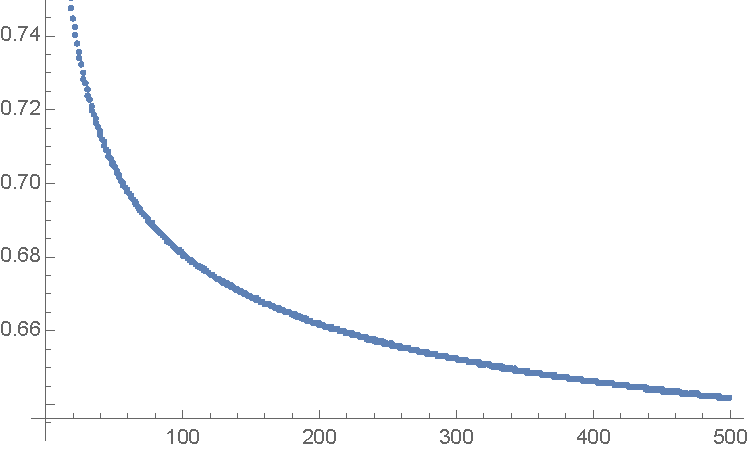
\includegraphics[scale=0.45]{../../Mathematica/alg-con-dom.pdf}
\end{minipage}
\end{frame}

\end{document}